\documentclass[paper.tex]{subfiles}

\begin{document}
\section{Introduction}
\label{sec:intro}

Quandles are algebraic structures that are deeply connected to knots. This connection is most strikingly presented by considering the arcs of a knot diagrams as objects acted on by the operation of
undercrossing, $\uc$. A set of axioms that $\uc$ must satisfy in order to be a `knot diagram invariant' (in a sense we will define shortly) can be easily derived from the Reidemeister moves, as shown in
Section~\ref{sec:quandle_axioms}.

But this is not the only way that quandles can be seen to be deeply connected to knots - associated with every knot is a `fundamental quandle'. This is obtained from the Wirtinger presentation of the fundamental knot group,
as the relations involve only conjugation (Section~\ref{sec:}). The fundamental quandle is nearly a complete knot invariant\footnote{It doesn't care about orientation}!


\subsection{Notation}

We set our notation for this manuscript in this section

\begin{itemize}
  \item We refer to the set of possible knot diagrams for a given knot $K$ as $\diag(K)$.
  \item We refer to the set of arcs in a knot diagram $d \in \diag(K)$ as $\A(d)$
  \item Let $\C(d)$ denote the set of crossings for a diagram $d$
  \item Let $\zeta_d: \C(d) \to \A(d) \times \A(d)$ denote the natural map that maps each crossing onto the pair of
    \emph{undercrossing} arcs. We require that $\zeta_d$ preserve order in the undercrossing arcs in the
    sense that if $a$ is an arc between crossings $c_1$ and $c_2$ then $\zeta_d(c_1) = (\alpha_1, a)$ and $\zeta_d(c_2) = (a, \alpha_2)$ for
    $\alpha_i \in \A(d)$. For instance, for a braid diagram (as in Figure~\ref{fig:braid_diagram}), the first element of $\zeta_d(c)$ is always the arc on the left of the crossing,
    and the second element is the arc on the right of the crossing.
  \item $\theta_i$ are projection maps onto the $i$th cartesian product. For instance, $\theta_1 \circ \zeta_d$ gives the first undercrossing arc.
  \item We denote the remainder of a number $n$ when divided by $k$ as $n\%k$.
  \item We denote $//$ to mean floor division.
\end{itemize}


\begin{figure}[h]
  \centering
  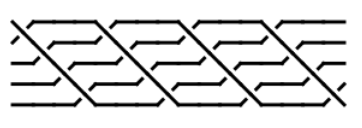
\includegraphics[width=0.7\textwidth]{braid_diagram}
  \caption{Example of a braid diagram}\label{fig:braid_diagram}
\end{figure}

\subsection{Quandles generalize $\Z_p$ coloring}

A \emph{$p$ coloring} of a knot diagram $d \in \diag(K)$ is a mapping $C: \A(d) \to \Z_p$ that does not map every arc onto a single element $p \in \Z_p$ and satisfies $z = 2x - y$ (in $\Z_p$) at each crossing where
$z$ is the label of the overcrossing and $x,y$ are the labels of the undercrossings. For $\Z_3$ for instance, this relation demands that either all three colors or only one of them are present at every crossing.

Quandles (we will get to their definition in a minute) can also be used to color knots. In fact, quandle coloring includes $\Z_p$ coloring as a special case (Section~\ref{sec:dihedral}). A \emph{quandle coloring} of a knot diagram
$d \in \diag(K)$ by a quandle $Q$ is a mapping $C: \A(d) \to Q$ such that the labeling rules as described in Figure~\ref{fig:labeling_rules} are satisfied at all crossings.

\begin{figure}[H]
  \centering
  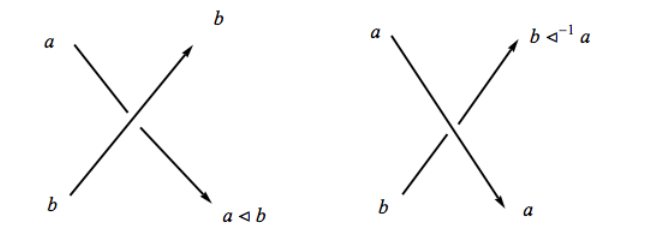
\includegraphics[width=0.8\textwidth]{labeling_rules}
  \caption{The convention we assume for quandle colorings. Figure reproduced from~\cite{Cusick}}\label{fig:labeling_rules}
\end{figure}


We say a knot is colorable by a quandle $Q$ if such a map $C: \A(d) \to Q$ satisfying the labeling rules exists. It so happens that for braid diagrams of $T(p,q)$ knots only the type of crossing on the left in
Figure~\ref{fig:labeling_rules} exists. This allows us to succintly express the colorability condition for $T(p,q)$ knots.

A braid diagram $b = {(B_p)}^q \in \diag(T(p,q))$ (Figure~\ref{fig:bp}) is colorable if $\forall c \in  \C(b) \theta_2 \circ \zeta_b(c) = \theta_1 \circ \zeta_b(c) \uc \theta_2 \circ \zeta_b(c)$.

Determining whether a given quandle $Q$ colors a knot $K$ is in general extremely difficult. In this work however, we restrict ourselves to a certain class of finite quandles (Section~\ref{sec:alexander}) as they have a very nice
form. This has the side effect that checking whether a quandle in this class colors a knot boils down to a mechanical procedure that gives an answer in finite (but possibly very large) time - everything is finite! Our contribution
in this work essentially just reduces the amount of computation that has to be done to check colorability through a careful treatment of the relations at hand.

One way to obtain a knot invariant from quandles is by counting the number of homomorphisms from the fundamental knot quandle into a fixed quandle $Q$. The Wirtinger has one generator for each arc in a knot diagram, so
this reduces to counting the number of quandle colorings in the sense we have just defined! To reiterate, if $Q$ admits $n$ colorings for a diagram of $K$ and $m \neq n$ colorings for $K^\prime$ then $K \not\cong K^\prime$.


\subsection{Deriving the quandle axioms from the Reidemeister moves}
\label{sec:quandle_axioms}

In this section we `derive' the quandle axioms from the Reidemeister moves, and in the process see how quandle colorings are naturally diagram invariants.

The first Reidemeister move (R1) allows to put in a `twist' on any arc of a knot diagram without changing its equivalency class. But putting in a twist introduces a crossing - so to make quandles R1 invariant we demand that
they satisfy $a \uc a = a$ for all $a \in Q$. See Figure~\ref{fig:r1} for a very helpful illustration.

R2 allows us to pull non-interesting strands away from each other. Figure~\ref{fig:r2} illustrates how this gives rise to the second axiom, that $(a \uc^{-1} b) \uc b = b$.

I will not attempt to describe R3. Figure~\ref{fig:r3} illustrates how it gives rise to the third axiom, that $(a \uc b) \uc c =  (a \uc c) \uc (b \uc c)$.

\begin{figure}[h]
  \centering
  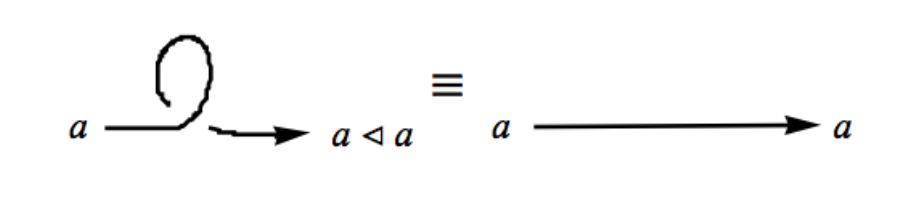
\includegraphics[width=0.8\textwidth]{R1}
  \caption{R1. Figure reproduced from~\cite{Cusick}. }\label{fig:r1}
\end{figure}

\begin{figure}[h]
  \centering
  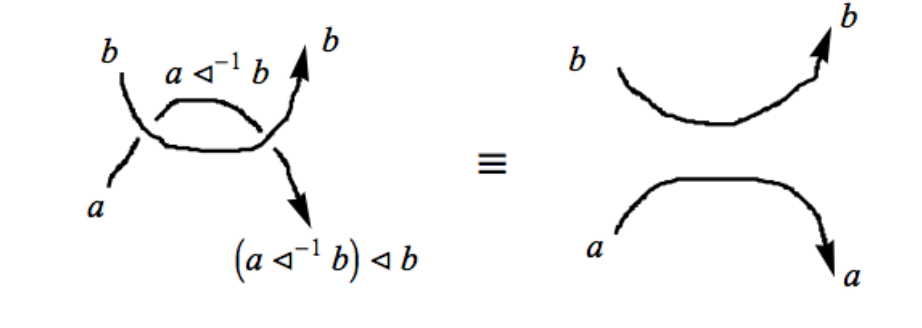
\includegraphics[width=0.8\textwidth]{R2}
  \caption{R2. Figure reproduced from~\cite{Cusick}.}\label{fig:r2}
\end{figure}

\begin{figure}[h]
  \centering
  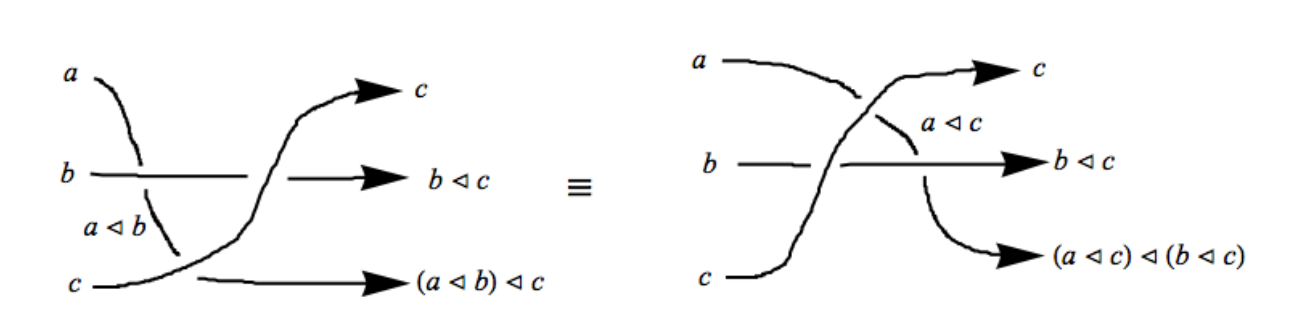
\includegraphics[width=0.8\textwidth]{R3}
  \caption{R3. Figure reproduced from~\cite{Cusick}. This picture is worth at least several hundred words.}\label{fig:r3}
\end{figure}



We can now give the definition of quandles.

\begin{definition}
An \emph{involutory quandle} is a set $K$ equiped with a binary operation $\uc$ such that $\forall x,y,z \in K$,

\begin{equation}
	x \uc x = x
\end{equation}
\begin{equation}
	(x \uc^{-1} y) \uc y = y \\
\end{equation}
\begin{equation}
	(x \uc y) \uc z = (x \uc y) \uc (x \uc z) \\
\end{equation}

We usually refer to this structure just as a quandle. They are called `involutory' because quandles are involutions (i.e. $\forall x \uc (x \uc x) = x$).

\end{definition}

\subsection{Classes of quandles}

In this section we give a very brief and not exhaustive description of some classes of Quandles.

\subsubsection{$\Z_{p,q}$ quandles}
\label{sec:alexander}

For any unit $q$ (fixed) in a commutative ring $K$, we can define a quandle structure over $K$, denoted by $K_q$, by setting

\begin{align}
  a \uc b &\defeq q a + (1 - q)b \\
  a \uc^{-1} b &\defeq q^{-1} a + (1 - q^{-1})b
\end{align}

In this work we concern ourselves with quandles of this type, taking $\Z_p$ as the base structure. We refer to this as a \emph{$\Z_{p,q}$ quandle}.

In general, quandles defined this way are called \emph{Alexander quandles}\footnote{Alexander quandles are constructed from modules over $\Z_p[t,t^{-1}]$ with $a \uc b \defeq t a + (1 - t) b$.}.

\subsubsection{Conjugal quandles}
\label{sec:conjugal}

We can define a quandle structure over any group $G$, using $n$-fold conjugation as the undercrossing operation.

\begin{equation}
  a \uc b \defeq b^n a b^{-n}
\end{equation}

\subsubsection{Dihedral quandles}
\label{sec:dihedral}

The order $n$ dihedral group $D_n$ gives rise to a quandle through conjugation, so dihedral quandles are a subset of conjugal quandles. However, they are notable for the following reason:
$\Z_{n, n - 1}$ gives rise to the same quandle! Furthermore, the dihedral undercrossing operation can be given as

$x\uc y \defeq 2x - y \mod n$

A knot is quandle colorable by the order $n$ dihedral quandle if and only if it is $\Z_n$ colorable! In this sense, $\Z_p$ coloring $\subset$ quandle coloring.


\end{document}
